\documentclass{beamer}

%% Juego de caracteres usado en el archivo fuente: UTF-8
\usepackage{ucs}
\usepackage[utf8x]{inputenc}
\uselanguage{spanish}
%Para la identación del español
\usepackage[spanish]{babel}

% There are many different themes available for Beamer. A comprehensive
% list with examples is given here:
% http://deic.uab.es/~iblanes/beamer_gallery/index_by_theme.html
% You can uncomment the themes below if you would like to use a different
% one:
%\usetheme{AnnArbor}
%\usetheme{Antibes}
%\usetheme{Bergen}
%\usetheme{Berkeley}
%\usetheme{Berlin}
%\usetheme{Boadilla}
%\usetheme{boxes}
%\usetheme{CambridgeUS}
%\usetheme{Copenhagen}
%\usetheme{Darmstadt}
%\usetheme{default}
%\usetheme{Frankfurt}
%\usetheme{Goettingen}
%\usetheme{Hannover}
%\usetheme{Ilmenau}
%\usetheme{JuanLesPins}
%\usetheme{Luebeck}
\usetheme{Madrid}
%\usetheme{Malmoe}
%\usetheme{Marburg}
%\usetheme{Montpellier}
%\usetheme{PaloAlto}
%\usetheme{Pittsburgh}
%\usetheme{Rochester}
%\usetheme{Singapore}
%\usetheme{Szeged}
%\usetheme{Warsaw}

%Para la identación del español
\usepackage[spanish]{babel}

\title{ModSecurity}

% A subtitle is optional and this may be deleted
%\subtitle{Optional Subtitle}

\author{Jesús Rodríguez Heras \\ Juan Pedro Rodríguez Gracia \\ Gabriel Fernando Sánchez Reina}
% - Give the names in the same order as the appear in the paper.
% - Use the \inst{?} command only if the authors have different
%   affiliation.

%\institute[Escuela Superior de Ingeniería] % (optional, but mostly needed)
%{
%  \inst{1}%
%  Department of Computer Science\\
%  University of Somewhere
%  \and
%  \inst{2}%
%  Department of Theoretical Philosophy\\
%  University of Elsewhere}
% - Use the \inst command only if there are several affiliations.
% - Keep it simple, no one is interested in your street address.

\date{31 de mayo de 2018}
% - Either use conference name or its abbreviation.
% - Not really informative to the audience, more for people (including
%   yourself) who are reading the slides online

%\subject{Theoretical Computer Science}
% This is only inserted into the PDF information catalog. Can be left
% out. 

% If you have a file called "university-logo-filename.xxx", where xxx
% is a graphic format that can be processed by latex or pdflatex,
% resp., then you can add a logo as follows:

% pgfdeclareimage[height=0.5cm]{university-logo}{university-logo-filename}
% \logo{\pgfuseimage{university-logo}}

% Delete this, if you do not want the table of contents to pop up at
% the beginning of each subsection:
%\AtBeginSubsection[]
%{
%  \begin{frame}<beamer>{Índice}
%    \tableofcontents[currentsection,currentsubsection]
%  \end{frame}
%}

% Let's get started
\begin{document}

\begin{frame}
  \titlepage
  
\end{frame}

\begin{frame}{Índice}
  \tableofcontents
  % You might wish to add the option [pausesections]
\end{frame}

% Section and subsections will appear in the presentation overview
% and table of contents.

\section{ModSecurity}
\subsection{Definición}
\begin{frame}{ModSecurity}
	\begin{block}{Definición}
		Es un motor de detección y prevención de intrusión de código abierto (Open Source) usado como firewall en aplicaciones web que permite detectar y bloquear ataques de tipo XSS y SQLi.
	\end{block}
\end{frame}

\subsection{Características}
\begin{frame}{ModSecurity}
\begin{block}{Características}
	La característica principal de ModSecurity es su capacidad de log y filtrado que permite almacenar el detalle de cada petición en un archivo de log que incluye los ``payloads'' de los POST HTTP. Los pedidos ofensivos serán rechazados o registrados según se configure.
\end{block}
\end{frame}

\section{Historia}
\begin{frame}{Historia}
	\begin{block}{Principios}
		Fue creado por Ivan Ristic en el año 2002 quien abordó el desarrollo de la aplicación después de haber utilizado durante un año y medio SNORT para monitorear el tráfico web y llegar a la conclusión de que necesitaba especificar más reglas.
	\end{block}
\end{frame}

\begin{frame}{Historia}
	\begin{block}{Desarrollo posterior}
		En el año 2006 Breach Security Inc adquirió ModSecurity y fue, a partir de este momento, donde el desarrollo de esta aplicación corrió por cuenta de esta empresa que le aportó mayores y mejores reglas en su implementación.
	\end{block}
\end{frame}

\section{Implementación}
\begin{frame}{Implementación}
	\begin{block}{Requisitos necesarios}
		Para la implementación de ModSecurity necesitamos lo siguiente:
		\begin{itemize}
			\item Servidor Apache en Debian.
			\item Apache ModSecurity.
		\end{itemize}
	\end{block}
\end{frame}

\begin{frame}{Servidor Apache en Debian}
	\begin{block}{Instalación y configuración}
		Para la instalación de Apache solo tenemos que introducir el siguiente comando en la terminal:
		\begin{center}
			\texttt{sudo apt-get install apache2}
		\end{center}
		Luego, entramos en el archivo \texttt{/etc/apache2/apache2.conf} y añadimos ``\texttt{ServerName www.trabajoASRC.com}'' para dotar a nuestro servidor de un nombre de dominio.
	\end{block}
\end{frame}

\begin{frame}{Servidor Apache en Debian}
\begin{block}{Cambiar DNS}
	Para poder acceder a nuestro servidor mediante el nombre de dominio previamente establecido accedemos la archivo ``\texttt{/etc/hosts}'' y agregamos ``\texttt{10.0.2.15 www.trabajoASRC.com}''.
\end{block}
\begin{alertblock}{IP y nombre de dominio}
	La IP asociada al nombre de dominio es \texttt{10.0.2.15} debido a que estamos trabajando con una máquina virtual con Debian.
\end{alertblock}
\end{frame}

\begin{frame}{Servidor Apache en Debian}
\begin{block}{Ejecutando Apache}
	Al iniciar el servidor con ``\texttt{/etc/init.d/apache restart}'', podemos ver que se ejecuta perfectamente con su correpsondiente nombre de dominio.
	\begin{center}
		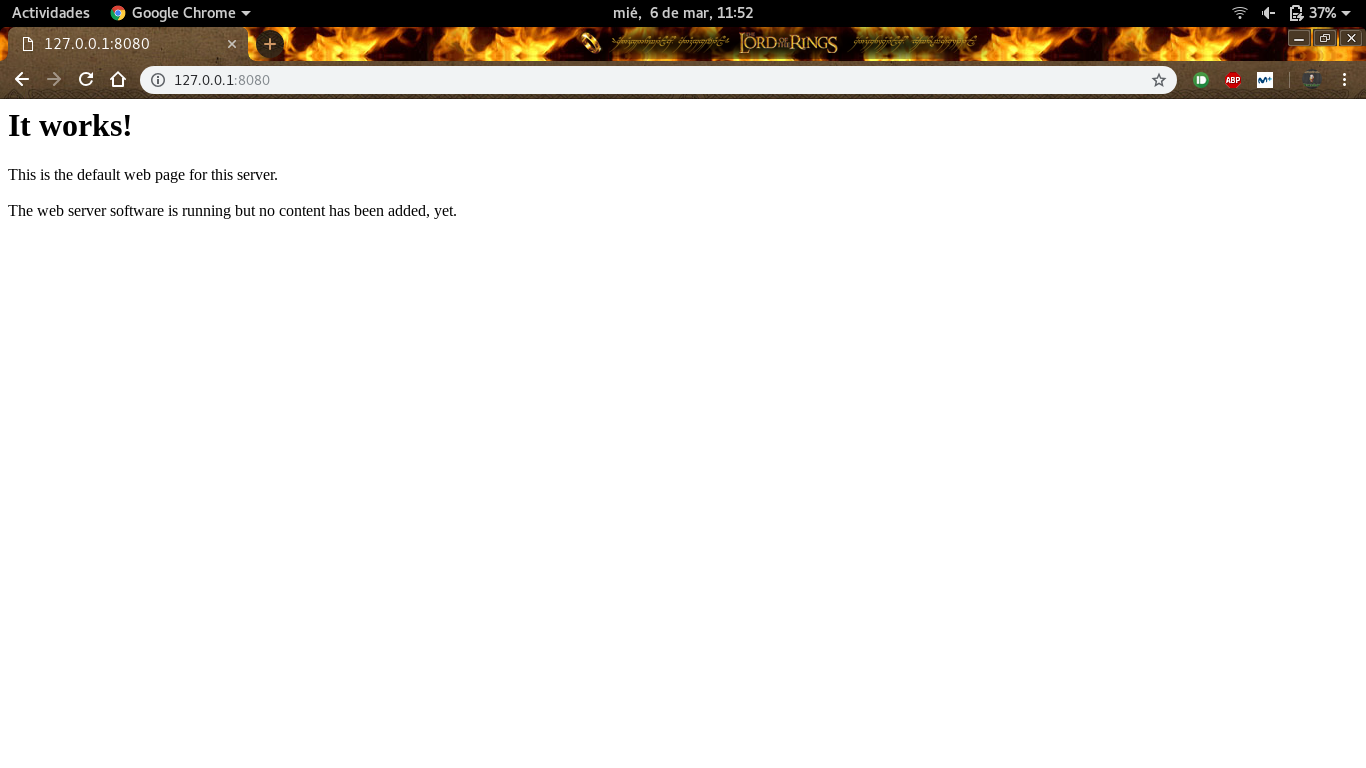
\includegraphics[scale=0.15]{apache.png}
	\end{center}
\end{block}
\end{frame}

\begin{frame}{Apache ModSecurity}
\begin{block}{Instalación}
	Para la instalación de Apache ModSecurity solo tenemos que introducir el siguiente comando en la terminal:
	\begin{center}
		\texttt{sudo apt-get install libapache2-modsecurity}
	\end{center}
	Lo que nos descargará e instalará correctamente la aplicación.
\end{block}
\end{frame}

\begin{frame}{Apache ModSecurity}
\begin{block}{Configuración}
	Para la configuración, nos dirigimos a ``\texttt{/etc/modsecurity}'' y, dentro de este directorio tendremos el archivo ``\texttt{modsecurity.conf}'' que será el que tengamos que ir modificando según lo que queramos que haga ModSecurity.
\end{block}
\end{frame}

\begin{frame}{Apache ModSecurity}
\begin{block}{Problemas configuración}
	Debido a que no tenemos los conocimientos necesarios sobre linux ni Apache, no hemos podido seguir, pero sí que hemos podido introducir algunas reglas en la configuración de ModSecurity:
	\begin{center}
		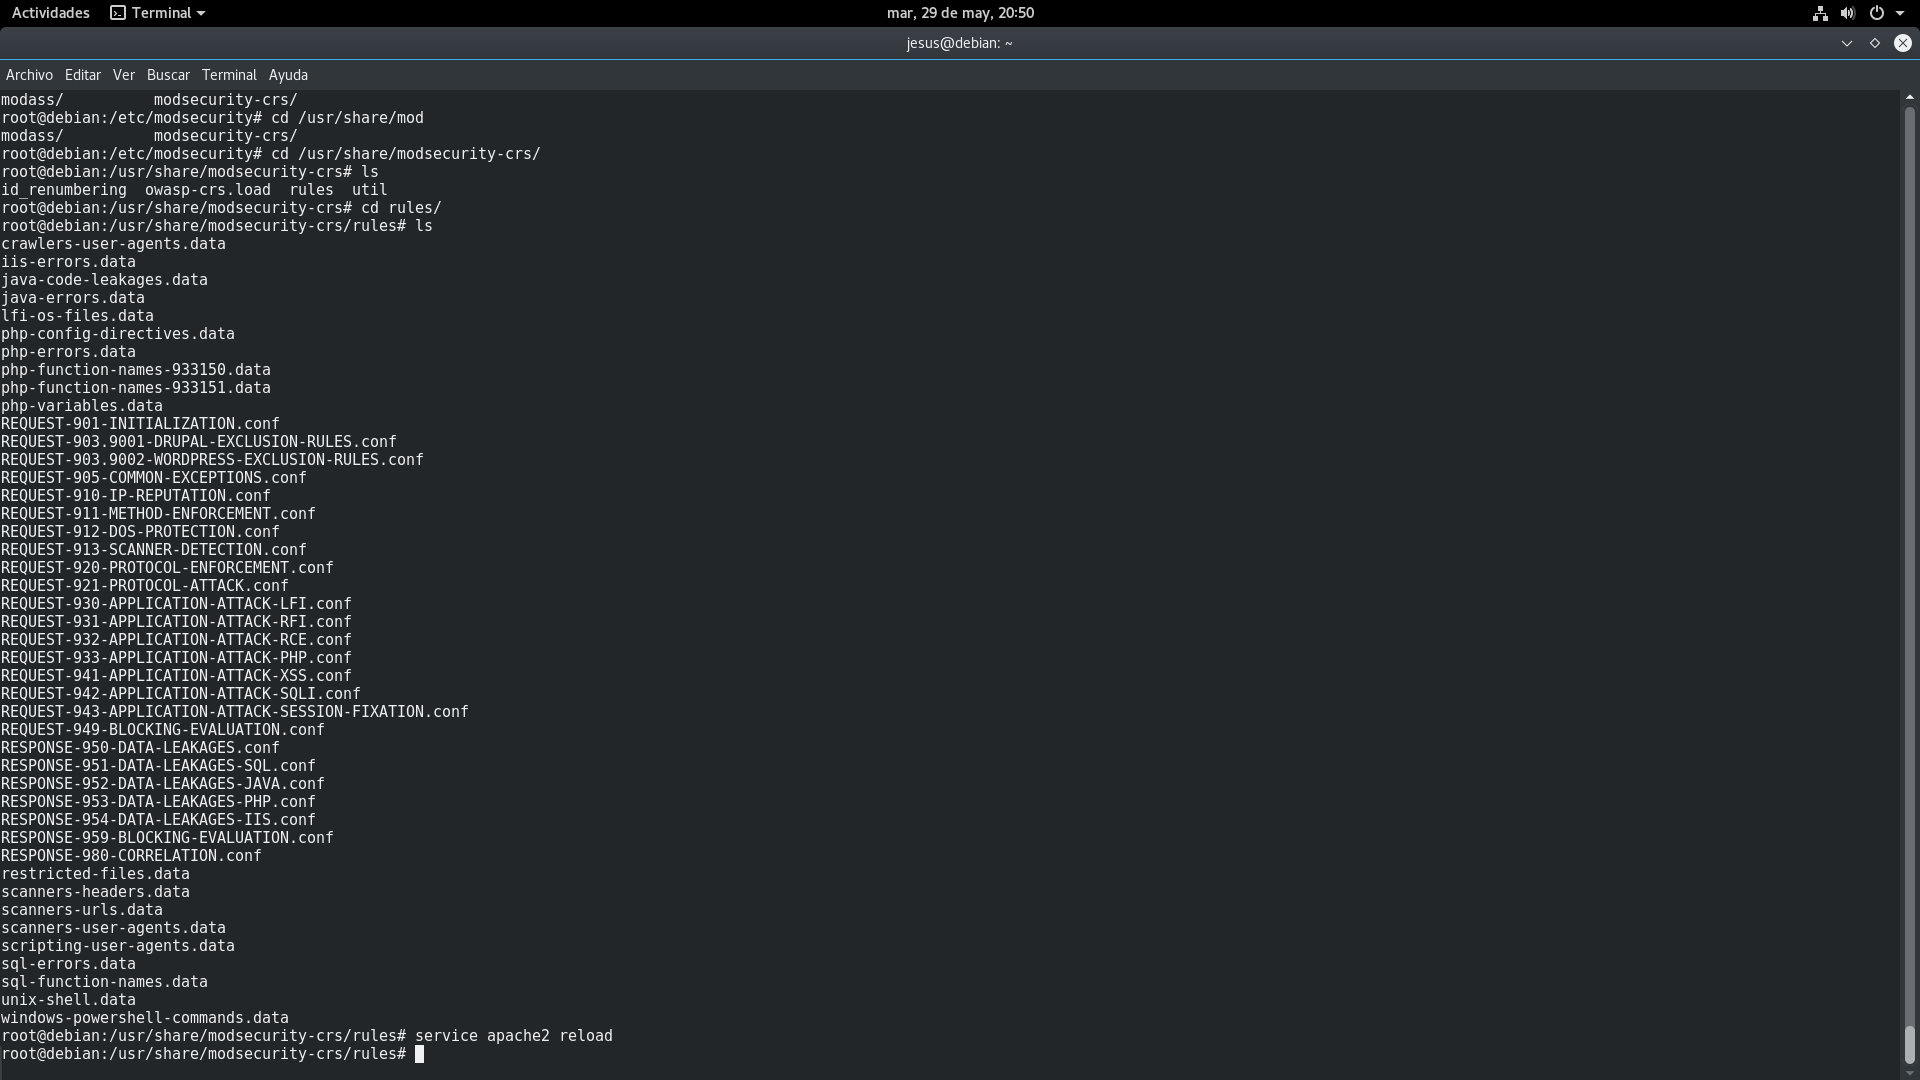
\includegraphics[scale=0.14]{reglas.png}
	\end{center}
\end{block}
\end{frame}



\end{document}


